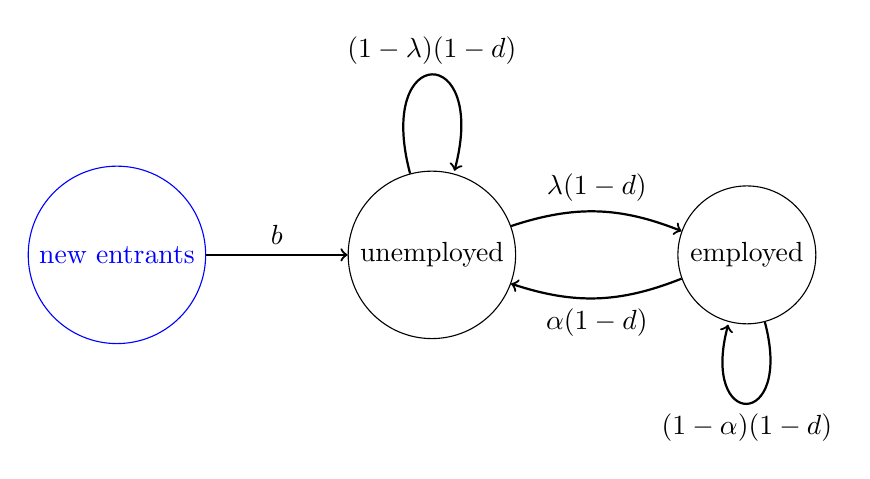
\begin{tikzpicture}
  \node[circle, draw] (1) at (-1, 0) {unemployed};
  \node[circle, draw] (2) at (3, 0) {employed};
  \node[circle, draw, blue] (3) at (-5, 0) {new entrants};
  \draw[->, thick, black]
  (1) edge [bend left=20, above] node {$\lambda (1-d)$} (2)
  (2) edge [bend left=20, below] node {$\alpha (1-d)$} (1)
  (2) edge [loop below] node {$(1-\alpha)(1-d)$} (2)
  (1) edge [loop above] node {$(1-\lambda)(1-d)$} (1)
  (3) edge [above] node {$b$} (1);
\end{tikzpicture}
